\section{Einleitung und Motivation}
%Wann und wo haben Sie Ihre Praxisphase absolviert?
%Wieso habe Sie diese Firma ausgewählt?
%In welchem Umfeld ist Ihre Praxisaufgabe?
%Welches Thema haben Sie gewählt? Warum?
%Besitzen Sie Vorkenntnisse, die Sie einbringen können?
%Gibt es Anknüpfungspunkte zum Studium am FB I?
Meine Praxisphase habe ich im Continental Konzern im Bereich der Basisentwicklung absolviert. 
In meiner Praxisphase wollte ich mein Wissen im Bereich der Entwicklung von Embedded Systems ausweiten und den Arbeitsalltag in einem großen Konzern kennen lernen. Continental war dafür genau richtig und bot mir eine Reihe von interessanten Themenvorschlägen an. 

Aus einer Auswahl von ca. 10 Praxisthemen, die mir Continental anbot und sich mit vielen verschiedene Teilaspekten der Softwareentwicklung für Embedded Systems beschäftigten, habe ich mich für das Thema "`sichere Kommunikation über das Controller Area Network"' entschieden, wobei ein Konzept über die Möglichkeiten und den Aufwand für eine sichere Kommunikation in den Netzwerk erstellt werden soll.
Dieses Thema beinhaltet neben Teilen aus dem Gebiet Embedded Systems auch Aspekte aus dem Feld der Kryptografie. In beiden Themen habe ich bereits in meinem Studium mehrere Vorlesungen belegt, die mein Interesse für die Fachgebiete geweckt haben. 
Außerdem finde ich die Erstellung eines Konzeptes sehr interessant, da es Spielraum für eigene Ideen und neue Ansätze bietet. 
%Anknüpfungspunkte???

\section{Das Unternehmen}
\subsection{Überblick}

%---
%Darstellung des Unternehmens (Industriezweig [ok], Sitz[ok], Personal- und Arbeitsstruktur ???
%Produkte [ok], Kunden [ok]) und wichtige Berufsfelder in der Firma (Kompetenzen, Ausbildung???)
%---

Die Continental Automitive AG ist ein Konzern der Automobilzuliefererbrache mit 190.000 Mitarbeitern, an über 200 Standorten und 53 Ländern. Der Hauptsitz befindet sich in Hannover. Neben dem ehemaligen Kerngeschäft, der Reifenproduktion, ist Continental einer der größten Automobilzulieferer weltweit. Zu den Kunden gehören neben allen großen deutschen Automobilherstellern weltweit viele namhafte Autokonzerne.


\subsection{Unternehmensbereiche (Divisionen)}

%---
%Organisationstruktur des Unternehmens [ok - nur erste Ebene], evtl. Zuordnung der Einheiten zu Produkte/Dienstleistungen
%---

Die Continental Automotive AG unterteilt sich in fünf Divisionen, die ich hier kurz vorstellen möchte. 

\paragraph{Chassis \& Safety}
Die Division Chassis and Safety entwickelt Fahrsicherheitssysteme, wie elektronische und hydraulische Bremssysteme, Sensorsysteme, sowie passive Sicherheitssysteme (z.B. Airbags) und Fahrassistenzsysteme (z.B. ABS) 

\paragraph{Powertrain}
Die Division Powertrain beschäftigt sich mit Lösungen rund um den Antriebsstrang von Fahrzeugen. Dazu gehören Komponenten für Motoren, Getriebe und Kraftstoffversorung, sowie mit dem Thema der Elektromobilität. 

\paragraph{Tires}
Die Division Tires ist mit der Entwicklung von Reifen für PKW und LKW befasst. 
\paragraph{ContiTech}
Die Division ContiTech spezialisiert sich auf Kautschuk und Kunststofftechnologie abseits der Reifen und hat zur Aufgabe Federungssysteme, Beförderungssysteme, Antriebsriemen, Membranstoffe, und außerdem Flüssigkeitstechnologien zu entwickeln. 

\paragraph{Interior}
Die Division Interior, der ich während der Praxisphase angehörte, fasst sämtliche Aktivitäten die das Darstellen und Auswerten von Informationen im Fahrzeug zusammen. Dabei steht die Schnittstelle zwischen Mensch und Maschine im Vordergrund.
Sie unterteilt sich in x Geschäftsbereiche Instrumentation and Driver HMI\footnote{"`Driver"' bezeichnet hierbei auf den Autofahrer und nicht, auf den Treiber im Sinne der Informatik}, Infotainment and Connectivity, 
%in der Infotainmentsystem entwickelt werden, 
Body and Security (Entwickung von Schließsystemen etc.), 
%die sich  mit Schließsystemen, sowie die Verfügbarkeit der Funktionen im Auto sicherstellt  und 
Commercial Vehicles \& Aftermarket (Bereich Nutzfahrzeuge und Vertrieb)
%die sich um spezifische Anforderungen im Bereich von Nutzfahrzeugen und Vertrieb kümmert.


%weitere unterpunkte für CDS Automotive etc. 


\subsubsection{Geschäfteinheit Instrumentation and Driver HMI}
%Zentrale Aufgaben 
In der Geschäfteinheit Instrumentation and Driver HMI geht es um die optische und grafische Aufbereitung und Vermittlung von Informationen, sowie die Entwicklung von innovativen Bedienelementen, die vom Fahrer während der Fahrt leicht abgelesen und bedient werden können. Hierfür werden sowohl einzelnen Komponenten, wie Kombiinstrumente, Sekundärdisplays und Head-up-Displays, als auch ganze Cockpitmodule entwickelt und hergestellt.

\subsubsection{Bereich Core Development Software}
Der Geschäftsbereiche '"Core Development Software (CDS)`" ist die zentrale, technologische Authorität im Geschäftseinheit Instrumentation \& Driver HMI. Die Hauptaufgabe besteht darin, die technologische Führereschaft des Geschäftsbereiches durch hohe Softwarequalität weiter auszuweiten. Dies geschieht durch Entwicklung bereits bestehender und neuer Softwarekomponenten und Plattformen, Forschung an neuen Technologien, Qualitätssicherung und Support beim Kunden.
Ziel ist es dem OEM eine einheitliche, sichere, fortschrittliche, skalierbare Plattform nach seinen Anforderungen zur Verfügung zu stellen, sodass diese mit einheitlichen Prozessen beim Kunden weiterentwickelt werden kann.
Das CDS umfasst die Technologien Grafik, HMI, Sound, Betriebsystem, Netzwerk, Treiber, Diagnose und Flash / Bootloader, der ich angehöre. 

\subsubsection{CDS Gruppe Flashbootloader} % Paragraph`??
Die Flashbootloader Gruppe beschäftigt sich mit der Entwicklung eines einheitlichen plattform- und technologieunabhägigen Flashprozesses und der Bereitstellung eines einfachen Systems zum Flashen von Systemen und Anwendungen für die Anwendungsentwicklung. 
Außerdem wird eine End-of-Line Diagnose bereitgestellt, die eine einfache Analyse des abgeschlossenen Fashprozesses zulässt. 
Weiter werden Software Pakete für Speichertechnologien für andere Teams bereitgestellt. 
%...


\subsection{Produkte}
%---
% Wichtige zentrale Produkte und Dienstleistungen, 
% insbesondere die darstellen, mit denen man direkt oder indirekt in Berührung kam oder die in der Abteilung unterstützt werden.
%---

Wie bereits im Punkt Unternehmensbereich beschrieben, entwickelt und fertigt Continental sehr viele verschiedene Komponenten und ganze Systeme für die Automobilindustrie. 
Besonders möchte dabei auf die Entwicklung von Kombiinstrumenten, Head-up Displays und ähnlichen informationstechnischen Komponenten eingehen, die von der Business Unit Instrumentation \& Driver HMI übernommen wird. 




%...

\subsection{Meine Praxisstelle - organisatorische Einbettung} % klingt scheiße

%---
% Wo ist die Stelle organisatorisch eingebettet? (Zu welchen anderen Organisationseinheiten bestehen kritische Abhängigkeiten?)
% Welche Aufgaben hat die Abteilung?
%In welchem Rahmen wurden Sie tätig? (Welche Aufgabenfelder wurden Ihnen übertragen?)
%---

% + erklären, warum ich im CDS sitze jedoch nichts mit denen direkt zu tun habe
Meine Praxisstelle habe ich wie bereits erwähnt am Standort Babenhausen absolviert, an dem die Kombiinstrumente, Head-up Displays und anderen HMI-Devices  entwickelt und gefertigt werden. 
Die Entwicklung wird am Standort Babenhausen in Verbindung mit den Standorten Singapur, Timisoara (Rumänien) und ferner Guadalajara (Mexiko) durchgeführt,  während die Fertigung ausschließlicn in Babenhausen stattfindet.
Dafür werden am Standort Babenhausen ca. 2.400 Mitarbeiter beschäftigt, wovon ca. 700 in der Entwicklung tätig sind. 

Für diese Komponenten werden in der Abteilung, in der ich tätig bin, Flashbootloader entwickelt. 
Meine Aufgabe hat zunächst nicht direkt etwas mit den primären Aufgaben Abteilung zu tun, in der ich sitze. Allerdings ist eine mögliche Schnittstelle über die der Flashvorgang stattfinden kann, das Controller Area Network CAN. Dieser Vorgang, der nicht nur im Werk, sondern auch beim Endkunden in einer Werkstatt stattfinden kann, soll gegen Eingriffe von außen abgesichert werden. Hieraus resultiert ein möglicher Anwendungsfall des von mir zu erstellende Konzept, für die Flash-Gruppe. 

\section{Das Projekt}
\unsure[inline]{ggf. einleitetenden Satz}
\subsection{Allgemeine Beschreibung}
% z.B. Was ist das Projektziel? 
% Wie heißt das Projekt? 
% Wer ist Auftraggeber?

Der Titel des von mir bearbeiteten Projektes lautet "`Sichere Kommunikation über das Controller Area Netzwork (CAN)"'. 
Ziel des Projektes ist es geeignete Mittel für ein sichere Kommunikation auszuwählen und den zusätzlichen Aufwand dafür abzustecken. Hierbei ist vor allem auf die Eignung im Umfeld von Embedded Systems zu achten. 
Das Projekt wurde Hausintern auf der Basis von Kundenanfragen generiert, die eine Absicherung sämtlicher Plattformen und Schnittstellen wünscht.
Die Ergebnisse des Konzeptes werden ggf. später in die Entwicklung neuer Flashprozesse einfließen oder als Sicherung der Kommunikation zwischen Komponenten im Auto eingesetzt werden.


\subsection{Meine Aufgabe} %ggf. redundant
% Darstellung der eigenen Aufgaben/Aufgabenbereiche 
% (was sollte entwickelt werden?)
% Architekturbilder, etc.

Meine Aufgabe ist es ein Konzept für eine sichere Kommunikation über das Controller Area Network (CAN) nach dem Stand der Technik zu erstellen. 

Die Aufgabe wurde zunächst sehr offen gehalten und beschrieb keine Wege oder einzusetzende Mittel. Es sollte von mir genauer recherchiert und beschrieben werden, was möglich und sinnvoll ist. Aufgrund der gewonnenen Erkenntnisse wurde die Aufgabe mit meinen Betreuern zusammen weiter eingegrenzt und präzisiert. 

Zu aktuellem Zeitpunkt ist die Aufgabe eine sichere M-N-Kommunikation aufzubauen, bei der alle Kommunikationspartner (Clients) gegenüber einem Server authentisieren müssen. Die Anzahl der Teilnehmer einer verschlüsselten Kommunikation soll zwischen zwei und dem durch das CAN-Netzwerk limitierte Maximum von 255 liegen. Es soll darüber hinaus möglich sein, zwei verschlüsselte Kommunikationen parallel und unabhängig von einander über einen Bus verschlüsselt unterhalten, wie in \autoref{fig:SichereKommunikation} gezeigt wird. 



\begin{figure}
\centering
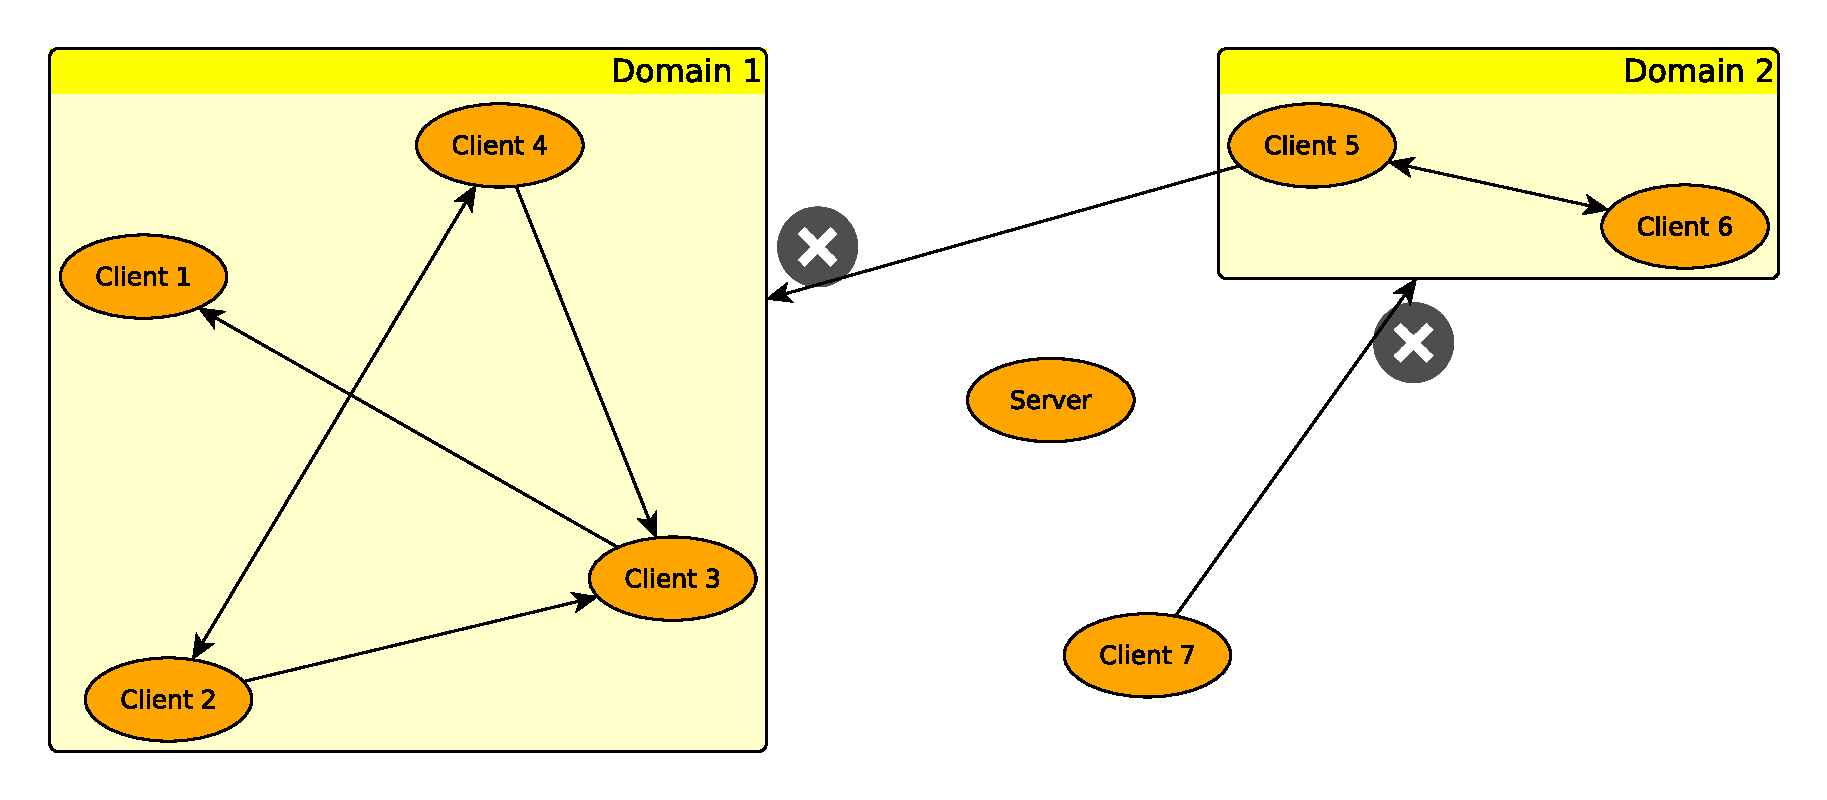
\includegraphics[width=0.8\textwidth]{Abb/Sichere_Kommunikation}
\caption[sichere Kommunikation]{Verschlüsselte Kommunikation in zwei Domänen}
\label{fig:SichereKommunikation}
\end{figure}

Zum aktuellem sollte die Beschreibung der Aufgabenstellung und somit auch der Umfang des Konzeptes weitestgehend Abgeschlossen sein und nur noch in Details verändert werden. Das Konzept wird, ggf. mit leicht reduziertem Inhalt, Thema meiner Bachelorarbeit mit dem gleichen Titel sein.


\subsection{Ziele}
Ziel meiner Praxisphase und der daraus resultierenden Bachelorarbeit ist es die Machbarkeit der sicheren Kommunikation über das CAN Protokoll zu beurteilen.

Dabei wurde mir ein sehr großer Spielraum bei der Aufgabenplanung und der Umsetzung gewährt. 

 Dazu sollen kryptografische Mittel nach aktuellem Stand der Technik ausgewählt und ein Vorschlag für ein Kommunikationsprotokoll gemacht werden, das eine für die Anwendungsschicht transparente Kommunikation gewährleistet. Die gewählten Ansätze sollen in Software umgesetzt werden und hinsichtlich Performance, Speicherverbrauch und Portabilität geprüft werden. Dabei sollen vor allem die Aspekte einer Instanzauthentifikation der Kommunikationsteilnehmer und eine Verschlüsselung der zu übertragenen Nachrichten betrachtet werden. 

\subsection{Eingesetzte Technologien}
%---
% Welche Technologien und Werkzeuge wurden eingesetzt?
% Was leisten die Werkzeuge?
%---
\unsure[inline]{ggf noch einleitenden Satz}
\paragraph{Netzwerk}
Zentraler Gegenstand meines Konzeptes ist das Controller Area Network CAN. \unsure{hier erklären?}

\paragraph{Testdevice}
Als Testdevice und die Aufnahme der Messwerte kommt im Moment nur ein BeagleBoneBlack zum Einsatz. Dieser wurde von Continental mit einer weiteren Platine ausgestattet, die 2 CAN Port bereitstellt und über GPIO PINs mit dem BeagleBone verbunden ist. 

 da das Portieren auf weitere Zielsysteme aus zeitlichen Gründen nicht mehr durchgeführt werden konnte. 
\paragraph{Betriebssystem}

Der Beagle Bone Black verfügt über ein Standard-Linux auf Basis einer Raspian Distribution, welche wiederum auf einem üblichen Debian Linux mit der Kernealversion 3.13 basiert. Die Wahl eines angepassten Desktop-Linux gegenüber einem "`echten"' embedded Linux, wie z.B. eines mit Yocto kompilierten Kernels, hat den Vorteil, dass es leichter angepasst werden kann. So können beispielsweise anderer Bibliotheken oder Updates einfach per aptitude installiert werden. 

Dies geht jedoch zulasten des Speicherverbrauches und der Zahl der laufenden Tasks und somit der Systemperformance, was jedoch auf dem BeagleBone keinen Einfluss auf die Messergebnisse haben sollte. 

\paragraph{Treiber}
 %überlegen ob hier erklären oder oben
\paragraph{Programmiersprachen}
Wie im embedded Umfeld üblich wurde der Prototyp in C / C++ entwickelt. Da ich einen CAN-Beispielprogramm in C++ zur Verfügung gestellt bekommen habe, jedoch die Anforderung hatte den Prototypen in C zu entwickeln, wurde die C++ Software auf zu portiert. 
Außerdem wurde C
\paragraph{Entwicklungswerkzeuge}
\subparagraph{Visual Studio}
Also Hauptentwicklungsumgebung kam zunächst Visual Studio zum Einsatz, da das Beispielprojekt bereits in Visual Studio vorlag und es bereits auf meinem Entwicklungs-PC vorinstalliert war
\subparagraph{Netbeans}
Da eine Cross-Plattform Entwicklung mit Visual Studio ohne weiteres nicht möglich ist, habe ich Netbeans als Entwicklungsumgebung speziell für Crossplattformentwicklung gewählt. Netbeans bietet eine sehr einfach Möglichkeit die Software für ein Target zu auf dem Host zu kompilieren. Das Ausführen und Debuggen geschieht auf dem Target, wobei die Darstellung in Netbeans integriert ist.\unsure{ggf. kürzen} %ggf. kürzen

\subparagraph{Enterprise Architect}
wurde  als Werkzeug zum Erstellen von UML Klassen- und Sequenzdiagrammen eingesetzt. Da bei der prototypischen Implementierung jedoch nicht unbedingt ein sauberes Softwaredesign im Vordergrund steht, wurde das Tool zur Visualisierung der Software bei Meetings eingesetzt. Aufgrund des hohen Zeitbedarfs der Pflege der Diagramme bin ich schnell aus Papier und Stift als Visualisierungsmittel ausgewichen.
\paragraph{Maketools und Compiler}
\subparagraph{Visual Studio Compiler}
%just for the record
Zunächst wurde der Visual Studio Compiler gewählt, da dieser auf dem Entwicklungsrechner vorhanden war. 

\subparagraph{GCC, mingw, make}
Als Compiler für das Target kam der GCC zum Einsatz, der auf Windows in Form von MinGW installiert wurde. 
GCC bietet mit GPROF  und GCOV umfangreiche Möglichkeiten zur Performancemessung von Quellcode. So kann beispielsweise die Zeit, die eine Methode zum durchlaufen benötigt gemessen werden und die CPU Auslastung gemonitored werden, ohne den Quellcode, etwa durch interne Timer, zu beeinflussen.
Zum kompilieren wurde ein Makefile erstellt, welches so aufgebaut wurde, dass die Messungen leicht integriert werden können und verschiedene Complieroptimierungen getestet werden können. 
Auf eine verwendung von CMake wurde aus zeitlichen Gründen verzichtet. 


\paragraph{Kryptografische Bibliotheken}
Ein großes Thema was mich durch den kompletten mittleren Teil meiner Praxisphase begleitet hat war die Auswahl einer kryptografischen Bibliothek um die Algorithmen bereit zu stellen.
\subparagraph{CryptoPP}Im C++ Projekt habe ich zunächst mit CryptoPP begonnen, da ich diese Bibliothek aus vorigen Arbeiten bereits kannte. Aufgrund von Einträgen in Internetforen habe ich angenommen, dass C-Bindings für CryptoPP existieren, was nicht der Fall ist. Somit war ein sinnvoller Einsatz von CryptoPP im C-Projekt unmöglich. 
\subparagraph{CryptLib}Als weitere Alternative recherchierte ich CryptLib, welche sich laut dem UserManual sehr gut für den Einsatz in embedded Systemen eignet. Die Einarbeitung in die Bibliothek erwies sich jedoch als derart kompliziert, dass ich von einer Verwendung absehen musste. 
\subparagraph{Hausinterne Bibliotheken}Auch ein Einsatz von Continental-internen Bibliotheken scheiterte an dem zu geringen Umfang dieser. 
\subparagraph{OpenSSL}Schließlich entschied ich mich für die Entwickler-API libcrypto, auf der OpenSSL basiert und die vom OpenSSL-Team entwickelt wird. Diese stellt alle relevanten Algorithmen, Verfahren und Parameter bereit und lässt sich einfach anwenden. Da der Prototyp nur darauf konzipiert ist auf dem BeagleBoneBlack zu laufen, der für ein embedded System relativ viel Performance besitzt, sind keine Einschränkungen Aufgrund der Bibliothek zu befürchten.


\subsection{Anforderungen}
%---
% Anforderungsanalyse (funktionale/nicht-funktionale Anforderungen)
%---
\paragraph{Funktionale Anforderungen}
\begin{itemize}
\item[] Zentrale Anforderung an die von mir zu erstellende prototypische Implementierung ist es eine belastbare Aussage darüber treffen zu können, ob es effizient möglich ist eine verschlüsselte und authentische Kommunikation beliebig vieler Teilnehmer über CAN durchzuführen und welche Mittel dafür eingesetzt werden müssen. 
\end{itemize}

\paragraph{Nichtfunktionale Anforderungen}
\begin{itemize}
	

\item Zeit zur Initiierung einer verschlüsselten Kommunikation soll den Systemstart und auch den Start der Netzwerkkumminikation nicht nennenswert verzögern.

\item Durch die verschlüsselte Kommunikation soll keine nennenswerten Verzögerungen in der Übertragung einer entstehen. Auch die Buslast soll sich nicht drastisch erhöhen.

\item Weiter ist eine wichtige Anforderung den Prototypen so zu entwickeln, dass er auf embedded Systems lauffähig ist. Besonders zu beachten ist dabei der Speicherverbrauch der Anwendung. 

\item Hinsichtlich der Implementierung ist eine Programmiersprache zu wählen, die weitreichende Kontrollmöglichkeiten bezüglich der Regeln der embedded Programmierung bietet.

\item Der Prototyp soll so plattformunabhängig, wie möglich gestaltet werden. Insbesondere bei der Auswahl der Bibliotheken ist dies zu beachten.

\item Kommunikationsprotokolle sollen leicht austauschbar gestaltet werden. 

\item Der Prototyp soll die Möglichkeiten von CAN voll ausnutzen können. Dabei sollen beliebig viele Teilnehmer beliebig vielen Untergruppen verschlüsselt kommunizieren können.

Weitere Anforderungen, z.B. was Bedienbarkeit, Konformität, Einhaltung von Softwarestandards, Wartbarkeit, Zuverlässigkeit oder Korrektheit angeht wurde im Rahmen der Anforderungsanalyse keine besondere Beachtung geschenkt, da es sich um eine prototypische Implementierung handelt. Diese müssen jedoch auch auf einem akzeptablen Niveau sein.

\end{itemize}

%Zuverlässigkeit (Systemreife, Wiederherstellbarkeit, Fehlertoleranz)
%nein Aussehen und Handhabung (Look and Feel)
%nein Benutzbarkeit (Verständlichkeit, Erlernbarkeit, Bedienbarkeit)
%OK Leistung und Effizienz (Antwortzeiten, Ressourcenbedarf, Wirtschaftlichkeit)
%OK Betrieb und Umgebungsbedingungen
%   Wartbarkeit, Änderbarkeit (Analysierbarkeit, Stabilität, Prüfbarkeit, Erweiterbarkeit)
%OK Portierbarkeit und Übertragbarkeit (Anpassbarkeit, Installierbarkeit, Konformität, Austauschbarkeit)
%?? Sicherheitsanforderungen (Vertraulichkeit, Informationssicherheit, Datenintegrität, Verfügbarkeit)
% nein Korrektheit (Ergebnisse fehlerfrei)
% nien Flexibilität (Unterstützung von Standards)
% OK Skalierbarkeit (Änderungen des Problemumfangs bewältigen)
%Randbedingungen

\subsection{Konzepte und Lösungsansätze}
%---
% Darstellung der Vorgehensweise sowie Lösung wichtiger Probleme, ...
%---

Um einen möglichst nachvollziehbaren Ansatz auszuwählen, habe ich mir zu Anfang meiner Praxisphase Gedanken darüber gemacht, welche Komponenten ich benötige, um die geforderten XXX umzusetzen. Die wichtigsten möchte ich im Folgenden kurz und so anschaulich, wie möglich erklären.

\subsubsection{Kommunikationsprotokoll}
Das CAN in einer Nachricht maximal nur 8 Byte an Daten übertragen kann, ist es unvermeidbar eine Art Kommunikationsprotokoll einzuführen, um längere Daten sinnvoll übertragen zu können. Um dies zu erreichen, habe ich zwei verschiedene Ansätze recherchiert, wovon ersterer Bestandteil der prototypischen Implementierung ist. 



\paragraph{Präfixprotokoll}
Beim Präfixprotokoll enthällt im ersten Byte des ersten Paketes die Anzahl der insgesamt zu übertragenen Bytes. Daraus entnimmt der Empfänger die Anzahl der zu sendenden Pakete und wartet bis alle eingetroffen sind. Nach der vollständigen Übertragung setzt er die Pakete wieder zu einer Nachricht zusammen.

Das Präfixprotokoll hat den Vorteil, dass man nur ein Byte an Protokolloverhead hat, jedoch den gravierenden Nachteil, dass nur eine endliche Menge von Daten übertragen werden kann, die vor der Übertragung bereits fest stehen muss. 
\paragraph{Streamprotokoll}
Im Streamprotokoll hingegen wird an den Anfang eines jeden Pakets ein Bit gesetzt, das signalisiert, ob ein weiteres Paket folgt, oder ob die Kommunikation abgeschlossen ist. 

Hier ist der Nachteil, dass in jedem Frame eine Protokolloverhead entsteht, jedoch lassen sich Nachrichten beliebiger Länge übertragen.


Optimierung hinsichtlich des verwendeten Protokolls, wie etwas hybride Verfahren der beiden Ansätze, sind denkbar. Da das Präfixprotokoll in aktueller Form, jedoch für den jetzigen Anwendungsfall ausreicht werden diese vorerst nicht weiter behandelt.
%\paragraph{Hybride Verfahren und Optimierungen}
%Denkbar sind außerdem hybride Verfahren, die beide Ansätze verbinden und weitere Optimierungen, wie etwa eine dynamische Ausweitung des Präfixprotkolls auf 

%Zu beachten ist, dass das man statt der Anzahl der zu übertragenen Bytes auch die Anzahl der folgenden Pakete übertragen könnten.

\subsubsection{Domänprinzip}

CAN folgt dem Multi-Master-Prinzieps, welches vereinfacht bedeutet, dass eine Nachricht an alle aktiven Teilnehmer versendet wird und die Empfänger aufgrund der CAN-ID (Identifikationsnummer einer Nachricht) entscheiden, welche für sie relevant ist. 

Um eine verschlüsselte M-N-Kommunikation via CAN durchzuführen, in der nur eine Teilmenge der Teilnehmer die Nachricht entschlüsseln kann, ist es erforderlich die Clients in Domänen zu unterteilen. Alle Teilnehmer erhalten nach der Authentifizierung vom Server den Schlüssel einer Domäne und können somit für sie bestimmte Nachrichten entschlüsseln, die aus der selben Domäne kommen.

\subsubsection{Authentifizierung}
In Absprache mit meinen Betreuern habe ich mich für eine Authentifizierung mit Hilfe einer Shared Secrets in Form einer Art Passworts entschieden. 

Dieses Passwort ist in den Hardwarebauteilen, in denen eine Implentierung der Software abläuft eine sogenannte DeviceID. Diese wird vom Hersteller hartcodiert, ist eindeutig und muss unter allen Umständen geheim gehalten werden. 

Der Hashwert dieser ID wird dem Server bei der Integration eines neuen Clients in das System auf einem sicheren Weg mitgeteilt
\footnote{Denkbar wäre hier z.B. eine Übertragung auf Dateibasis per USB, dies war jedoch nicht die Aufgabe meiner Praxisphase}.

Bei der Anfrage einer sicheren Kommunikation sendet der Client diese DevicID verschlüsselt mit einem zuvor ausgehandeltem, asymmetrischem Authentifizierungsschlüssel und in Form eines Hashwerts an den Server, welcher dieses mit dem gespeicherten Passwort abgleicht.

Ist diese Authentifizierung erfolgreich bekommt der Client den symmetrischen Schlüssel, verschlüsselt mit einem asymmetrischen Verschlüsselungsschlüssel, welchen er entschlüsseln und verwenden kann. 

\subsubsection{Verschlüsselung}
Die Verschlüsselung der Nachrichten, geschieht über ein symmetrisches Verschlüsselungsverfahren. Der hier für benötigte Schlüssel wird nach der Authentifizierung mit einem zuvor ausgehandeltem, asymmetrischem Schlüssel verschlüsselt übertragen. Alle Clients der Domain verwenden den selben Schlüssel und können die gesendeten Nachrichten somit entschlüsseln. 

Zu beachten ist hierbei, dass um die Backward- und Foreward-Security \footnote{Anschaulich: Ein ,fälschlicher weise, bereits authentisierter potenzieller Angreifer, kann mit dem erhaltenen Schlüssel keine Informationen der vorangegangenen und kommenden Sitzung entschlüsseln} zu gewährleisten, bei jeder Aufnahme eines neuen Client der Verschlüsselungsschlüssel aller Client der Daomain ausgetauscht wird. 

\subsubsection{Messungen}
Zum Messen der Performance der von mir erstellten, prototypischen Implementierung kommt, wie bereits erwähnt die GPROF-Erweiterung des GCC-Kompilers zum Einsatz. 
\todo{ausweiten oder weglassen}

\subsection{Aktueller Stand} 
% was wurde realisiert?
Zum aktuellen Zeitpunkt ist die Auswahl von, für Testzwecke sinnvollen, kryptografischen Algorithmen und einer Bibliothek, die diese bereit stellt abgeschlossen. 

Eine prototypische Implementierung, ist ebenfalls nahezu abgeschlossen. Diese Erfüllt die meisten, gestellten Anforderungen, jedoch können anhand dieser momentan nur Messungen einer 1-1-Kommunikation durchgeführt werden. 

Des Weiteren konnte der Prototyp fast vollständig auf ein embedded Linux portiert werden.

Außerdem wurden Betrachtungen zum einer perfekten Sicherheit\unsure{hab ich das eigentlich irgendwo oben erwähnt?} durchgeführt und skizzenhaft festgehalten. 



\subsection{Bewertung des Ergebnisses} 
%ggf. redundant zu unten
Auch wenn das Konzept zum aktuellen Zeitpunkt noch nicht Abgeschlossen ist, kann ich ein überwiegend positives Resümee meiner Praxisphase ziehen\unsure{kann ich das so schreiben?}. 
Neben einer Analyse und einer inhaltlichen Eingrenzung, war ich in der Lage einen Prototypen zu erstellen, der den meisten gestellten Anforderungen gerecht wird und Messungen, der Performance und der Nachrichtenlaufzeiten zulässt. 

Eine von mir zu spät erkannte Schwierigkeit ist die saubere Trennung der CAN-IDs während der Authentifizierung, weshalb der Prototyp aktuell nur in einer 1-1-Kommunikation funktioniert. Dies wird jedoch im Rahmen meiner Bachelorarbeit noch ausgebessert.

Neben der Implementierung der Prototypen, der keine Umfassende Sicherheit bietet, war ich in der Lage eine begründete Skizze zu erstellen, welches optimale Sicherheit nach dem Stand der Technik bietet. Außerdem habe ich mich mit den Eigenschaften der verschiedenen kryptografischen Verfahren beschäftigt und geeignete Algorithmen und Parameter ausgewählt.

In Bezug auf die Auswahl einer kryptografischen Bibliothek hätte eine intensivere Auseinandersetzung mit den in Frage kommenden Bibliotheken und eine schnellere Rücksprache mit Know-How-Trägern einiges an Zeit gespart. 

Die Portierung der Software von Windows auf Linux, scheiterte zunächst an Hardware- und Toolproblemen, welche nun jedoch gelöst sind, sodass die Implementierung jetzt auf den BeagleBone mit dem embedded Linux portiert werden kann.

Angesichts des aus meiner Sicht sehr großen Umfangs der Praxisphase konnte ich nichts desto trotz bereits relativ viel umsetzen\unsure{klingt das zu eingebildet?}.

\subsection{Ausblick}
Da meine Praxisphase noch nicht ganz beendet ist und das Thema Bestandteil meiner Bachelorarbeit sein wird, möchte ich noch einen kurzen Ausblick geben. 

Nachdem nun eine funktionierende Entwicklungsumgebung zum Cross-Kompilieren aufgebaut werden konnte, muss der Prototyp auf den BeagleBone portiert werden, wofür nicht mehr als 3 Tage vorgesehen sind. 

Danach werden erste von Messungen auf dem Zielsystem durchgeführt und mit Hilfe der gewonnen Erkenntnissen wird der Prototyp weiter optimiert. 

Anschließend sollte noch eine Erweiterung der Implementierung auf eine M-N-Kommunikation stattfinden, welche eine weiter Messreihe nach sich zieht.

Eine Betrachtung auf unterschiedlichen Zielsystemen, wie z.B. dem JCP2011 und Betriebssystemen (Linux, Autosar os, QNX) steht noch aus. Dazu muss die Software jedoch noch den jeweiligen Einschränkungen der Plattformen und Betriebssystemen angepasst werden, was einiges an Zeit und Know-How erfordert. Dies wird im Rahmen meiner Arbeit an dem Projekt voraussichtlich nicht mehr statt finden. 

\section{Evaluation der Praxisphase}
\subsection{Die Aufgabe}
%eigener Punkt
Die von mir für meine Praxisphase gewählte Aufgabe hat sich als äußerst interessant, jedoch aber auch als wesentlich umfangreicher als zunächst angenommen herausgestellt. 

Der Ansatz einer sehr offenen Fragestellung bot mir  viele Möglichkeiten im Studium erlernte Methoden anzuwenden, aber auch eigene Ideen einzubringen. Die Präsentation meiner Ergebnisse und das Diskutieren meiner Ansätze mit meinen Betreuern und Experten war hierbei, jedoch absolut notwendig, um das Ergebnis so aussagekräftig, wie möglich zu gestalten.
%ggf. noch interessantes Forshcungsgbiet generell bla.



\subsection{Das Unternehmen als Praxisstelle}
%Wie verlief das Praktikum? Gab es Probleme? Wurden Sie gut betreut?
%Wie war das Arbeitsklima? Was war bei der Firma besonders interessant?
%Gab es besondere Angebote bzgl. Weiterbildung?

%- meetings
Insgesamt verlief meine Praxisphase bei Continental sehr gut. Das Arbeitsumfeld war angenehm, mir wurden die benötigten Arbeitsmaterialien schnell zur Verfügung gestellt und ich hatte viele Freiheiten während meiner Arbeitszeitw, wie z.B. Arbeitszeiten aus Gleitzeitbasis und die Möglichkeit bestimmte Arbeiten im Homeoffice durchzuführen. 
Bei Bedarf bzw. wöchentlichen Meetings mit meinen Betreuern [Betreuer klingt irgendwie doof] konnte ich meine Fortschritte vorstellen und aufgrund neuer Erkenntnisse veränderte Anforderungen mit ihnen durchsprechen. Meine Betreuer auch den Kontakt zu Experten bestimmter Gebiete her, die mir bei der Problemlösung behilflich waren. 

% - alleiniger frickler
Da ich die Aufgabe meiner Praxiphase alleine bearbeitete hatte ich leider nicht so viel fachlichen Austausch mit den Kollegen in meinem Büro, die mit anderen Aufgaben befasst waren. Dies war jedoch aus den bereits beschriebenen Gründen nicht anders möglich.

%- keine Prozesse für Crosscompile 
Außerdem waren die Auflagen des IT-Services hinsichtlich Anpassungen von Programmen und Betriebsystemen teilweise sehr störend. Vor allem der Aufbau einer einfachen, soliden Crosscompiler Toolchain von einem Windows Host auf eine Embedded Linux Target war nahezu unmöglich und kostete viel Zeit.


\subsection{Lessons Learned}
%eigener Punkt
Der größte und wichtigste Punkt, den ich in meiner Praxisphase gelernt habe, ist, dass es extrem schwierig ist die Erstellung eines Konzeptes sinnvoll zu planen. 
Während der Recherche entstehen immer neue Fragen, Probleme und Optimierungsansätze, aufgrund dessen die Beschreibung des Konzeptes weiter angepasst und verfeinert werden muss. 
Hierbei den Überblick zu behalten, alle Anforderungen und Erkenntnisse sinnvoll zu beschreiben und einzuordnen und dabei Fortschritte zu machen erfordert viel Disziplin. %klingt scheiße --> verbessern

Außerdem musste ich mehrere "Technologiebrüche" überwinden, die durch eine umsichtigere Planung unter Umständen vermeidbar gewesen wären. So habe ich zum Beispiel die Entwicklung auf der Basis eines CAN-Beispielprogramms begonnen, welches als Visual Studio Projekt vorlag und einen properitäten Vector-Treiber\footnote{Die Vector Informatik GmbH ist der Hersteller der von uns verwendeten CAN-Hardware.} enthielt und in C++ geschrieben war. Dies musste im Laufe der Zeit auf ein in C geschriebenes, makefile-basiertes Projekt mit dem Linux-CAN-Open Treiber portiert werden, was einiges an Zeit in Anspruch nahm. 
Außerdem musste ich mich, wie bereits beschrieben sehr lange mit der Wahl einer kryptografischen Bibliothek beschäftigen.

\subsection{Persönliche Einschätzung des Lernerfolgs}
%Lernerfahrungen, Stellenwert der praktischen Erfahrungen im Rahmen des Studiums,
%Auswirkungen der gesammelten Erfahrungen auf die eigenen beruflichen Pläne, andere persönliche
%Überlegungen, die im Zusammenhang mit dem Praktikum entstanden sind.

In meiner Praxisphase konnte ich viele Erfahrungen sammeln, die im Studium in dieser Art und Weise natürlich nicht vermittelt werden können. 

Allein die Bearbeitung einer umfangreichen Aufgabenstellung über einen längeren Zeitraum und die damit verbundene intensive Auseinandersetzung mit den Themen waren für mich komplett neu. 

Auch die Arbeit in einem Großkonzern habe ich als überwiegend positiv wahrgenommen, auch wenn natürlich Abstriche in der Flexibilität und den Tools gemacht werden mussten. Dafür hatte ich eine sehr große Wissensbasis zur Verfügung und konnte auf das Know-how viele Experten zurückgreifen. 

Das Thema meiner Praxisphase finde ich schon seit langem sehr interessant. Die Praxisaufgabe hat mich in meinem Interesse für die Themen embedded Systems und Kryptografie bestätigt, sodass ich mich wahrscheinlich in Zukunft weiter diesen Themen widmen werde. 


%Abkürzungsverzeichnis brauche ich wohl nicht 

% Glossar 

%Quellennachweis / Literaturverzeichnis
% kann aus dem Expose genommen und leicht angepasst werden 
